% ==============================================================================
% CAPÍTULO 9: RESULTADOS Y DISCUSIÓN
% ==============================================================================
\section{RESULTADOS Y DISCUSIÓN}

En este capítulo se presentan los resultados obtenidos tras la ejecución del banco de pruebas experimental sobre la Máquina Virtual de Java (JVM), abarcando las condiciones reales de ejecución, el análisis estadístico descriptivo e inferencial, las distribuciones gráficas de latencia y memoria, y la discusión frente a la literatura previa.

\subsection{Ejecución del protocolo y entorno controlado}

Las pruebas se realizaron sobre una estación de trabajo de escritorio con procesador AMD Ryzen 5 3400G (4 núcleos físicos / 8 hilos a $3.70\text{ GHz}$), placa base MSI A320M-A PRO (MS-7C51), $16.0\text{ GB}$ de memoria física instalada ($13.9\text{ GB}$ utilizables) y sistema operativo Microsoft Windows 11 Pro de 64 bits (compilación 26300). Para reducir el ruido derivado de la planificación de procesos en segundo plano, el equipo operó bajo el perfil energético de alto rendimiento y sin aplicaciones de usuario activas durante la ventana de medición.

Para garantizar igualdad de condiciones en la ocupación espacial, los tres formatos se evaluaron bajo un mismo paradigma de materialización completa en memoria antes de ejecutar el conteo de registros: matriz tabular residente en Heap (\texttt{List<List<String>{}>}) para CSV, modelo de árbol de objetos (\texttt{JsonNode} de Jackson) para JSON y árbol jerárquico estándar W3C DOM (\texttt{org.w3c.dom.Document}) para XML \cite{w3cdom2004}. El banco experimental ejecutó los 18 escenarios ($3\text{ formatos} \times 2\text{ niveles de profundidad} \times 3\text{ volúmenes nominales}$) con semilla determinista (\texttt{Random(42)}), asegurando equivalencia semántica estricta de $6\,500$, $65\,000$ y $325\,000$ registros. Cada escenario incluyó 5 iteraciones previas de calentamiento del compilador JIT seguidas de 30 repeticiones instrumentadas, completando 540 mediciones válidas en 5 minutos y 40 segundos sin errores de agotamiento de memoria.

El $100\%$ de las corridas superó la validación automática de conteo de registros en memoria. Durante la auditoría de ejecución se registraron tres precisiones metodológicas:
\begin{itemize}
    \item \textbf{Versión de la máquina virtual:} Si bien el marco de referencia partió de la especificación Java SE 21, el entorno real corrió sobre OpenJDK 25.0.4.1 (64-Bit Server VM) utilizando el recolector G1GC predeterminado.
    \item \textbf{Gestión del espacio Heap:} La JVM operó con su límite ergonómico por defecto de $3\,566\text{ MB}$ de Heap máximo, holgura suficiente para sostener sin degradación las estructuras en memoria de mayor tamaño ($95.97\text{ MB}$ en disco).
    \item \textbf{Depuración de valores atípicos:} Al aplicar el filtro de rango intercuartílico de Tukey ($Q_{1} - 1.5 \times \text{IQR}$ y $Q_{3} + 1.5 \times \text{IQR}$) sobre la latencia por escenario, se conservaron 493 observaciones y se descartaron 47 puntos extremos ($8.7\%$) asociados a interrupciones transitorias del sistema operativo.
\end{itemize}

\subsection{Estadística descriptiva: peso sintáctico, latencia y memoria}

La etapa de generación evidenció la penalización espacial que introduce la verbosidad sintáctica antes siquiera de iniciar el análisis en memoria. Para una carga idéntica de $325\,000$ registros, CSV ocupó $23.45\text{ MB}$ en disco en ambos esquemas; por el contrario, JSON demandó $56.92\text{ MB}$ (plano) y $65.60\text{ MB}$ (anidado), mientras que XML escaló hasta $81.72\text{ MB}$ (plano) y $95.97\text{ MB}$ (anidado), más de cuatro veces el tamaño del archivo tabular.

\begin{table}[htbp]
\centering
\caption{Estadística descriptiva de tiempo de procesamiento y memoria Heap en estructura plana (1 nivel).}
\label{tab:desc_plano}
\resizebox{\textwidth}{!}{%
\begin{tabular}{llccccccc}
\toprule
\textbf{Volumen} & \textbf{Formato} & \textbf{$n$} & \textbf{Disco (MB)} & \textbf{Tiempo Media $\pm$ DE (ms)} & \textbf{Mediana / IQR (ms)} & \textbf{RAM Pico (MB)} & \textbf{RAM Retenida (MB)} & \textbf{Factor $\alpha$} \\
\midrule
\multirow{3}{*}{1 MB}  & CSV  & 24 & 0.46  & $8.88 \pm 0.62$     & $9.01 / 0.75$     & 5.13   & 3.34   & $7.29\times$ \\
                       & JSON & 30 & 1.13  & $17.74 \pm 4.12$    & $18.26 / 8.05$    & 7.64   & 6.07   & $5.38\times$ \\
                       & XML  & 29 & 1.62  & $48.08 \pm 2.38$    & $47.73 / 3.41$    & 16.48  & 11.68  & $7.19\times$ \\
\midrule
\multirow{3}{*}{10 MB} & CSV  & 26 & 4.64  & $44.12 \pm 4.72$    & $43.22 / 6.21$    & 41.39  & 33.29  & $7.18\times$ \\
                       & JSON & 29 & 11.33 & $159.97 \pm 16.69$  & $166.89 / 21.18$  & 93.76  & 60.53  & $5.34\times$ \\
                       & XML  & 25 & 16.29 & $307.03 \pm 11.12$  & $305.97 / 6.09$   & 161.80 & 116.64 & $7.16\times$ \\
\midrule
\multirow{3}{*}{50 MB} & CSV  & 30 & 23.45 & $247.03 \pm 22.73$  & $248.67 / 33.26$  & 232.55 & 166.89 & $7.12\times$ \\
                       & JSON & 27 & 56.92 & $633.39 \pm 26.16$  & $623.35 / 34.52$  & 383.64 & 303.30 & $5.33\times$ \\
                       & XML  & 27 & 81.72 & $1468.89 \pm 42.79$ & $1468.18 / 52.59$ & 777.38 & 582.37 & $7.13\times$ \\
\bottomrule
\end{tabular}%
}
\end{table}

Como detalla la Tabla~\ref{tab:desc_plano} para estructuras planas de $50\text{ MB}$ nominales, el análisis sintáctico y construcción completa del árbol W3C DOM en XML demandó en promedio $1\,468.89\text{ ms}$, superando en $5.95$ veces el tiempo de CSV ($247.03\text{ ms}$) y en $2.32$ veces el de JSON ($633.39\text{ ms}$). Respecto a la huella espacial, el factor de expansión ($\alpha = M_{\text{RAM}} / S_{\text{disco}}$) se mantuvo estable en torno a $5.33\times$ para el modelo de árbol de JSON y $7.13\times$ para el árbol DOM de XML.

\begin{table}[htbp]
\centering
\caption{Estadística descriptiva de tiempo de procesamiento y memoria Heap en estructura anidada (3 niveles).}
\label{tab:desc_anidado}
\resizebox{\textwidth}{!}{%
\begin{tabular}{llccccccc}
\toprule
\textbf{Volumen} & \textbf{Formato} & \textbf{$n$} & \textbf{Disco (MB)} & \textbf{Tiempo Media $\pm$ DE (ms)} & \textbf{Mediana / IQR (ms)} & \textbf{RAM Pico (MB)} & \textbf{RAM Retenida (MB)} & \textbf{Factor $\alpha$} \\
\midrule
\multirow{3}{*}{1 MB}  & CSV  & 27 & 0.46  & $8.84 \pm 0.21$     & $8.83 / 0.24$     & 5.16   & 3.33   & $7.28\times$ \\
                       & JSON & 29 & 1.30  & $23.99 \pm 6.48$    & $28.05 / 11.88$   & 9.66   & 8.65   & $6.65\times$ \\
                       & XML  & 27 & 1.91  & $47.43 \pm 1.29$    & $47.04 / 1.67$    & 16.97  & 12.67  & $6.64\times$ \\
\midrule
\multirow{3}{*}{10 MB} & CSV  & 23 & 4.64  & $40.91 \pm 1.66$    & $40.74 / 2.39$    & 41.99  & 33.27  & $7.17\times$ \\
                       & JSON & 27 & 13.07 & $209.19 \pm 11.77$  & $210.59 / 11.56$  & 118.31 & 86.35  & $6.61\times$ \\
                       & XML  & 28 & 19.14 & $351.79 \pm 18.35$  & $354.94 / 25.81$  & 171.17 & 126.30 & $6.60\times$ \\
\midrule
\multirow{3}{*}{50 MB} & CSV  & 30 & 23.45 & $247.39 \pm 22.66$  & $252.13 / 27.33$  & 236.57 & 166.89 & $7.12\times$ \\
                       & JSON & 27 & 65.60 & $794.65 \pm 37.16$  & $783.04 / 34.03$  & 494.38 & 432.27 & $6.59\times$ \\
                       & XML  & 28 & 95.97 & $1684.39 \pm 44.24$ & $1678.43 / 62.29$ & 827.57 & 629.64 & $6.56\times$ \\
\bottomrule
\end{tabular}%
}
\end{table}

Al introducir tres niveles de jerarquía (Tabla~\ref{tab:desc_anidado}), la penalización computacional se acentúa en los modelos basados en árbol. En el escenario crítico de $50\text{ MB}$ anidados, el árbol DOM de XML alcanza una latencia media de $1\,684.39\text{ ms}$ ($6.81$ veces más lento que CSV) y una ocupación retenida de $629.64\text{ MB}$ con picos transitorios de $827.57\text{ MB}$ en Heap. En JSON, la incorporación de subobjetos \texttt{ObjectNode} eleva su factor de expansión $\alpha$ de $5.33\times$ a $6.59\times$, incrementando en un $42.5\%$ su consumo de RAM retenida respecto a la versión plana.

\subsection{Presentación gráfica de distribuciones}

La distribución completa de las 493 observaciones limpias se ilustra mediante diagramas de caja para el tiempo de procesamiento (Figura~\ref{fig:tiempo_boxplots}) y la memoria Heap retenida (Figura~\ref{fig:ram_boxplots}). Mientras que la latencia exhibe rangos intercuartílicos acotados con leve dispersión por planificación de hilos, la memoria retenida presenta varianza prácticamente nula ($\text{DE} < 0.43\text{ MB}$ en todos los escenarios), confirmando el determinismo estructural de la instanciación de nodos en el Heap.

\begin{figure}[htbp]
    \centering
    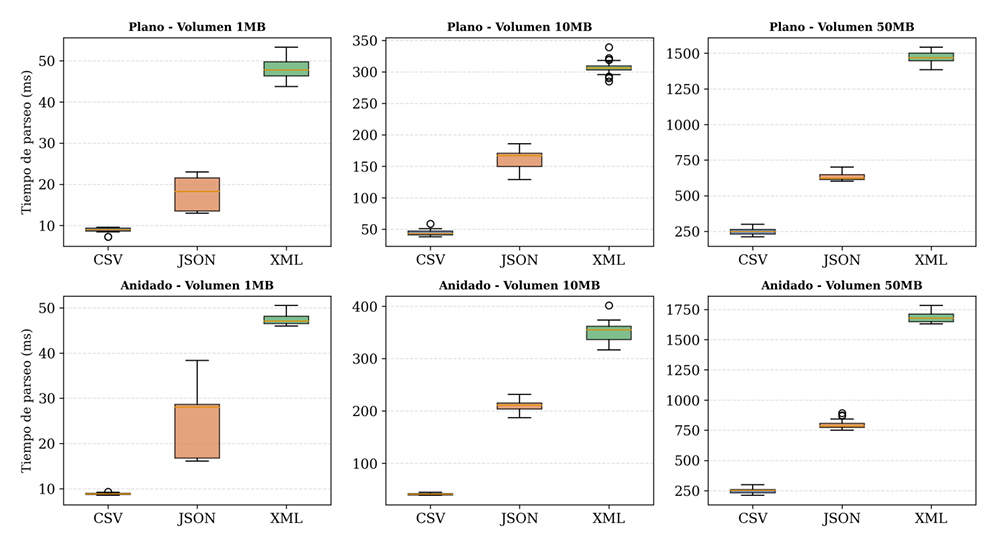
\includegraphics[width=\textwidth]{fig_tiempo_boxplots.png}
    \caption{Distribución del tiempo de procesamiento (ms) en los 18 escenarios experimentales tras el filtrado por IQR. Se observa el escalamiento respecto al volumen y la separación entre CSV, JSON y XML.}
    \label{fig:tiempo_boxplots}
\end{figure}

\begin{figure}[htbp]
    \centering
    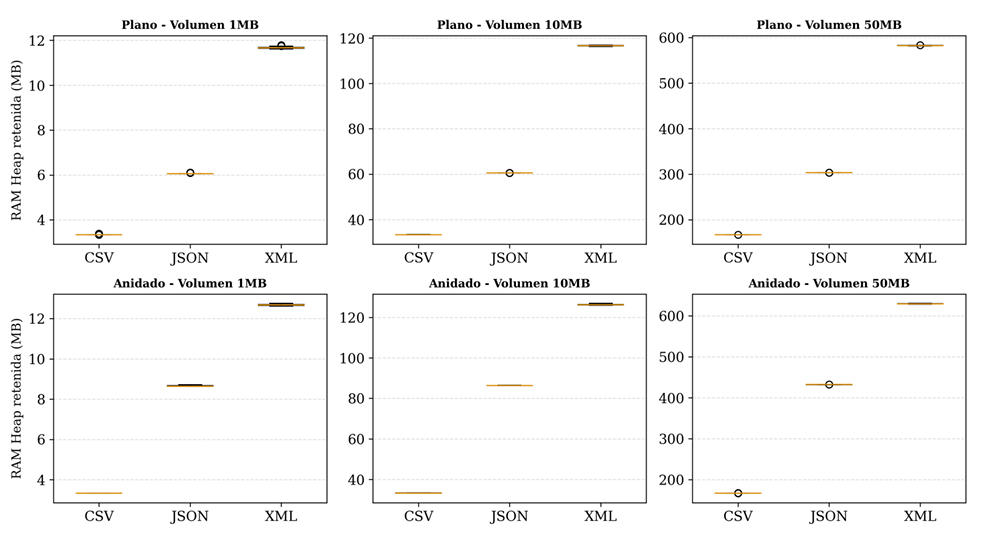
\includegraphics[width=\textwidth]{fig_ram_boxplots.png}
    \caption{Distribución de la memoria Heap retenida (MB) tras la materialización completa en memoria. La ausencia de dispersión vertical evidencia la huella determinista de cada modelo de objetos.}
    \label{fig:ram_boxplots}
\end{figure}

\subsection{Estadística inferencial y contrastación de hipótesis}

La verificación previa de normalidad mediante la prueba de Shapiro-Wilk ($\alpha = 0.05$) reveló desviaciones significativas respecto a la distribución normal en los grupos de memoria retenida (debido a su carácter determinista) y asimetrías moderadas en latencia. En consecuencia, se aplicó la prueba no paramétrica de Kruskal-Wallis ($H$) para contrastar el efecto del formato entre CSV, JSON y XML, complementada con ANOVA de una vía ($F$) en el único bloque estrictamente normal (tiempo de parseo en esquema anidado de $10\text{ MB}$), y la prueba $U$ de Mann-Whitney con $d$ de Cohen para evaluar el impacto de la profundidad jerárquica.

\begin{table}[htbp]
\centering
\caption{Contrastación inferencial entre formatos (CSV, JSON y XML) y tamaños del efecto por escenario.}
\label{tab:inferencial}
\resizebox{\textwidth}{!}{%
\begin{tabular}{llccccc}
\toprule
\textbf{Escenario} & \textbf{Métrica Evaluada} & \textbf{Prueba Aplicada} & \textbf{Estadístico} & \textbf{Valor $p$} & \textbf{Tamaño del Efecto} & \textbf{Decisión ($\alpha = 0.05$)} \\
\midrule
\multirow{2}{*}{Plano 1 MB}   & Tiempo de parseo & Kruskal-Wallis & $H = 72.66$ & $1.67 \times 10^{-16}$ & $\epsilon^{2} = 0.886$ & Rechaza $H_{0}$ \\
                              & RAM retenida     & Kruskal-Wallis & $H = 75.13$ & $4.85 \times 10^{-17}$ & $\epsilon^{2} = 0.916$ & Rechaza $H_{0}$ \\
\midrule
\multirow{2}{*}{Plano 10 MB}  & Tiempo de parseo & Kruskal-Wallis & $H = 70.13$ & $5.92 \times 10^{-16}$ & $\epsilon^{2} = 0.888$ & Rechaza $H_{0}$ \\
                              & RAM retenida     & Kruskal-Wallis & $H = 70.32$ & $5.36 \times 10^{-16}$ & $\epsilon^{2} = 0.890$ & Rechaza $H_{0}$ \\
\midrule
\multirow{2}{*}{Plano 50 MB}  & Tiempo de parseo & Kruskal-Wallis & $H = 73.72$ & $9.83 \times 10^{-17}$ & $\epsilon^{2} = 0.888$ & Rechaza $H_{0}$ \\
                              & RAM retenida     & Kruskal-Wallis & $H = 73.72$ & $9.83 \times 10^{-17}$ & $\epsilon^{2} = 0.888$ & Rechaza $H_{0}$ \\
\midrule
\multirow{2}{*}{Anidado 1 MB} & Tiempo de parseo & Kruskal-Wallis & $H = 72.87$ & $1.50 \times 10^{-16}$ & $\epsilon^{2} = 0.889$ & Rechaza $H_{0}$ \\
                              & RAM retenida     & Kruskal-Wallis & $H = 76.76$ & $2.15 \times 10^{-17}$ & $\epsilon^{2} = 0.936$ & Rechaza $H_{0}$ \\
\midrule
\multirow{2}{*}{Anidado 10 MB}& Tiempo de parseo & ANOVA ($F$)    & $F = 3589.43$ & $3.50 \times 10^{-75}$ & $\eta^{2} = 0.990$     & Rechaza $H_{0}$ \\
                              & RAM retenida     & Kruskal-Wallis & $H = 68.68$ & $1.22 \times 10^{-15}$ & $\epsilon^{2} = 0.892$ & Rechaza $H_{0}$ \\
\midrule
\multirow{2}{*}{Anidado 50 MB}& Tiempo de parseo & Kruskal-Wallis & $H = 74.62$ & $6.25 \times 10^{-17}$ & $\epsilon^{2} = 0.888$ & Rechaza $H_{0}$ \\
                              & RAM retenida     & Kruskal-Wallis & $H = 74.62$ & $6.25 \times 10^{-17}$ & $\epsilon^{2} = 0.888$ & Rechaza $H_{0}$ \\
\bottomrule
\end{tabular}%
}
\end{table}

\textbf{Resolución de las hipótesis planteadas:}
\begin{itemize}
    \item \textbf{Hipótesis sobre tiempo de procesamiento ($H_{1a}$):} Se rechaza la hipótesis nula $H_{0a}$ en los seis bloques volumen-estructura ($p < 10^{-15}$). Los tamaños del efecto obtenidos ($\epsilon^{2} \ge 0.886$ y $\eta^{2} = 0.990$, muy por encima del umbral clásico de efecto grande de $0.14$) confirman que cerca del $89\%$ de la varianza en latencia responde directamente al formato de serialización, validando que CSV presenta tiempos significativamente inferiores a JSON y XML en todos los escenarios.
    \item \textbf{Hipótesis sobre consumo de memoria RAM ($H_{1b}$):} Se rechaza la hipótesis nula $H_{0b}$ en todos los bloques evaluados ($p < 10^{-14}$, $\epsilon^{2} \ge 0.888$). XML exhibe un consumo de memoria Heap pico y retenida significativamente superior a JSON y CSV para volúmenes de datos equivalentes. Adicionalmente, al contrastar esquemas planos frente a anidados en $50\text{ MB}$ mediante la prueba $U$ de Mann-Whitney, CSV no mostró diferencias significativas ($p = 0.935$ en tiempo, $d = +0.02$; $p = 0.853$ en RAM), mientras que la jerarquía incrementó significativamente el costo en JSON ($+25.5\%$ en tiempo, $p = 3.03 \times 10^{-10}$, $d = +5.02$; $+42.5\%$ en RAM) y en XML ($+14.7\%$ en tiempo, $p = 2.08 \times 10^{-10}$, $d = +4.95$; $+8.1\%$ en RAM).
\end{itemize}

\subsection{Discusión frente a la literatura y alcance del estudio}

Los resultados experimentales dialogan directamente con los hallazgos previos sobre serialización e intercambio de datos en entornos administrados:
\begin{itemize}
    \item \textbf{Sobrecarga del modelo DOM en XML:} La penalización medida en XML (hasta $6.81\times$ en tiempo y $3.77\times$ en memoria frente a CSV) respalda lo documentado en evaluaciones recientes sobre estándares de almacenamiento estructurado \cite{ieee_les_2024, ieee_parsing_2008} respecto al costo del análisis léxico de etiquetas redundantes de apertura y cierre, así como el sobrecosto espacial de instanciar cada elemento y nodo de texto como objetos independientes en el Heap de la JVM \cite{dke_memory_2006, oracle_jvm_spec}.
    \item \textbf{Asimetría entre tamaño en disco y expansión en memoria en JSON:} Trabajos centrados en eficiencia de transmisión suelen destacar la compacidad de JSON frente a XML \cite{ieee_les_2024, maltsev2024b}. Los datos obtenidos matizan esa ventaja al trasladar el análisis a la memoria de la JVM: aunque JSON plano exhibe el menor factor de expansión ($\alpha \approx 5.33\times$), la introducción de jerarquías anidadas multiplica la creación de contenedores \texttt{ObjectNode} en Jackson, elevando su expansión a $\alpha \approx 6.59\times$ y equiparándola proporcionalmente con XML anidado ($\alpha \approx 6.56\times$).
    \item \textbf{Estabilidad estructural del formato CSV:} Frente a la degradación observada en los formatos jerárquicos, CSV conserva un costo invariante ante el anidamiento lógico ($p = 0.935$) al proyectar la jerarquía mediante encabezados compuestos, ratificando su eficiencia en procesos de ingesta masiva homogénea señalada en la literatura de análisis de alto rendimiento \cite{ieee_icoailo_2025, langdale2019}.
\end{itemize}

\textbf{Limitaciones y amenazas a la validez:} De acuerdo con el diseño metodológico, tres condiciones acotan la generalización de estos resultados sin afectar su validez interna: en primer lugar, los tiempos absolutos en milisegundos están ligados al procesador AMD Ryzen 5 3400G y a la implementación de OpenJDK 25, aunque las proporciones relativas entre formatos derivan de la arquitectura interna de cada analizador; en segundo lugar, el experimento se circunscribió a estrategias de materialización completa en memoria (\texttt{Document}, \texttt{JsonNode} y colecciones tabulares), por lo que no abarca el comportamiento de analizadores secuenciales basados en flujo de eventos (SAX, StAX o Jackson Streaming); finalmente, los conjuntos de datos sintéticos emplearon esquemas regulares homogéneos, dejando fuera documentos con alta irregularidad estructural o cargas binarias incrustadas.